\scanpage{84}
\mspage{83}
Soit d'autre part
\[
A=\{z_1,z_2\}
\]
on aura donc
\[
|A|=|z_1|\cup|z_2|=\{x_1,x_2,x'_1,x'_2\unsure{)|\}}
\]
mais $\operatorname{supp}A=A_{z_1}\vee A_{z_2}$ donc
\[
|\operatorname{supp}A|=[x_1,x_2]\unsure{\vee|\cup}[x'_1,x'_2]
\]
\unsure{il y a} donc
\[
|A|\subsetneq|\operatorname{supp}A|.
\]
Considérons \unsure{le} $z_3=(x_3,x'_3)$ avec
\[
\begin{aligned}
x_1<x_3<x_2,\\
x'_2<x'_3<x'_1
\end{aligned}
\]
et
\[
\begin{aligned}
A_{z_3}\cap(A_{z_1}\vee A_{z_2})&=A_{z_3}\\
(\underbrace{A_{z_3}\cap A_{z_1}}_{\varnothing})\vee(\underbrace{A_{z_3}\cap A_{z_2}}_{\varnothing})&=\varnothing
\end{aligned}
\]
donc on n'a pas la propriété modulaire de distributivité de $\cap$ p.r. à $\vee$ !

\uline{Conclusion}-\uline{Scholie} Le formalisme des supports est bon, \deleted{(en dehors des cas} pourvu qu'on ne s'avise pas de comparer les supports des strates et des figures \deleted{\unsure{pas, qui ne soient}} \inserted{qui ne soient} compatibles, ou qui ne puissent l'être moyennant subdivision. (Tel est le cas des \unsure{miens|miens,} en dehors de la situation quasi-ensembliste, ou \unsure{plus génl.|plus général.}, la situation formelle dégagée page $80$.)
% Double vertical emphasis strokes alongside the conclusion.
\margin{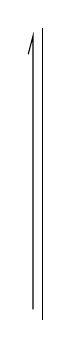
\begin{tikzpicture}\draw (0,.03)--(0,3.5)--(-.06,3.27);\draw (.12,-.1)--(.12,3.6);\end{tikzpicture}}
